\begin{frame}
	\frametitle{From the View of Learning Data}
	\begin{figure}
		\centering
		\begin{tikzpicture}
		\path (0,0) pic[scale=0.5] {unlabeled};
		\path (0,0) pic[scale=0.5] {labeled};
		
		\node[note] at (1.8,1.8) {Semi-supervised learning (SSL)};
		\end{tikzpicture}
		\caption*{Labeled with a large amount of unlabeled data}
	\end{figure}

	\vspace{-.5cm}
	\pause
	\begin{figure}
		\centering
		\begin{subfigure}[b]{0.45\textwidth}
			\centering
			\begin{tikzpicture}
			\pic[scale=0.4] at (0,0) {unlabeled};
			\pic[scale=0.4] at (0,0) {labeled};		
			\draw[orange] (1.5,-.3) -- (2,1.3) node[midway, sloped, above, inner sep=1pt, orange]{\scriptsize classifier};
			\end{tikzpicture}
			\caption*{Discriminative: Direct solution}
		\end{subfigure} 
		\hfill
		\begin{subfigure}[b]{0.45\textwidth}
			\centering
			\begin{tikzpicture}
			\node[fill=orange, opacity=.5, ellipse, minimum height=45pt, minimum width=60pt](re1) at (.7,.5) {};
			\node[fill=blue, opacity=.5, ellipse, minimum height=50, minimum width=50, right of=re1, xshift=.8cm] {};
			
			\path (0,0) pic[scale=0.4] {unlabeled};
			\path (0,0) pic[scale=0.4] {labeled};	
			\end{tikzpicture}
			\caption*{Generative: Data boundary}
		\end{subfigure}
	\end{figure}
\end{frame}

\begin{frame}
	\frametitle{Outline}
	\begin{block}{Multinomial Naive Bayes}
		\begin{itemize}
			\item Inductive learning
			\item A class is constructed of many sub-components  
			\item How do we initialize these sub-components?
			\item Apply on text data
		\end{itemize}
	\end{block}
\end{frame}

\begin{frame}
	\frametitle{Component Assumptions}
	Given a component set $M$, we have
	\begin{align*}
		P(x) = \sum_{M_j \in M}P(x|M_j)P(M_j)
	\end{align*}
	with predefined $P(y|M_j) \in \{0, 1\}$
	
	\pause
	\vspace{.5cm}
	\begin{block}{Many-to-one assumption}
		\begin{figure}
			\centering
			\begin{subfigure}[b]{0.4\textwidth}
				\centering
				\begin{tikzpicture}[scale=.3]
				% default mu=0
				\newcommand \SIGMA{1};
				\newcommand \SHIFT{3*\SIGMA};
				\newcommand \SHIFTT{10*\SIGMA};
				
				\begin{axis}[
				hide y axis,
				axis x line*=bottom,
				xticklabels={}
				]
				\addplot [draw, ultra thick, domain=-3*\SIGMA-\SHIFT:3*\SIGMA-\SHIFT,samples=201] {gauss(-\SHIFT, \SIGMA)};
				\addplot [draw, ultra thick, domain=-3*\SIGMA+\SHIFT:3*\SIGMA+\SHIFT,samples=201] {gauss(\SHIFT, \SIGMA)};
				
				\addplot [draw, ultra thick, domain=-3*\SIGMA-\SHIFTT:3*\SIGMA-\SHIFTT,samples=201] {gauss(-\SHIFTT, \SIGMA)};
				\addplot [draw, ultra thick, domain=-3*\SIGMA+\SHIFTT:3*\SIGMA+\SHIFTT,samples=201] {gauss(\SHIFTT, \SIGMA)};
				\end{axis}
				\end{tikzpicture}
				\caption*{$P(x)$}
			\end{subfigure}
			\begin{subfigure}[b]{0.4\textwidth}
				\centering
				\begin{tikzpicture}[scale=.3]
				% default mu=0
				\newcommand \SIGMA{1};
				\newcommand \SHIFT{3*\SIGMA};
				\newcommand \SHIFTT{10*\SIGMA};
				
				\begin{axis}[
				hide y axis,
				axis x line*=bottom,
				xticklabels={}
				]
				\addplot [fill=red, opacity=.5, domain=-3*\SIGMA-\SHIFT:3*\SIGMA-\SHIFT,samples=201] {gauss(-\SHIFT, \SIGMA)};
				\addplot [fill=blue, opacity=.5, domain=-3*\SIGMA+\SHIFT:3*\SIGMA+\SHIFT,samples=201] {gauss(\SHIFT, \SIGMA)};
				
				\addplot [fill=red, opacity=.5, domain=-3*\SIGMA-\SHIFTT:3*\SIGMA-\SHIFTT,samples=201] {gauss(-\SHIFTT, \SIGMA)};
				\addplot [fill=blue, opacity=.5, domain=-3*\SIGMA+\SHIFTT:3*\SIGMA+\SHIFTT,samples=201] {gauss(\SHIFTT, \SIGMA)};
				\end{axis}
				\end{tikzpicture}
				\caption*{$P(x|y)$}
			\end{subfigure}
		\end{figure}
	\end{block}
\end{frame}

\begin{frame}
	\frametitle{How Do We Initialize These Components?}
	Conventional methods set it randomly
	\begin{align*}
		P(M_j|y) \sim \mathcal{U}(0,1) \quad \textnormal{such that} \quad \sum_{M_j:P(y|M_j)=1}P(M_j|y) = 1
	\end{align*}
	
	\begin{columns}[t]
		\column{0.55\textwidth}
		In this way, it assumes that
		\begin{itemize}
			\item All components are the same 
			\item Different outputs when we re-sampling 
		\end{itemize}
	
		\pause[2]
		\rule{\textwidth}{1pt}
	
		\textcolor{blue}{Or it better to be seen as an unsupervised task}
		\begin{itemize}
			\item Consider the structure of data
			\item Keep the same samples when re-sampling
		\end{itemize}
		
		\pause[0]
		\column{0.5\textwidth}
		\vspace{-.7cm}
		\begin{figure}
			\centering
			\begin{subfigure}[b]{\textwidth}
				\centering
				\begin{tikzpicture}[scale=.7]
				\node[vertex](v1) at (1, 0) {};
				\node[vertex, draw=none, inner sep=0] at (2, 0) {$\dots$};
				\node[vertex](v2) at (3, 0) {};
				\node[vertex](v3) at (4, 0) {};
				
				\node[fill=orange!40, minimum size=15pt](c1) at (1.5, -2){};
				\node[fill=orange!40, minimum size=15pt](c2) at (3.5, -2){};
				
				\draw[->] (v1)--(c1);
				\draw[->] (v1)--(c2);
				\draw[->] (v2)--(c1);
				\draw[->] (v2)--(c2);
				\draw[->] (v3)--(c1);
				\draw[->] (v3)--(c2);
				
				\node[fill=none, dashed, draw, ellipse, right of=v1, 
				minimum width=80pt, minimum height=20pt](e1){};
				\node[fill=none, dashed, draw, ellipse, right of=c1, 
				minimum width=80pt, minimum height=25pt, xshift=-.3cm](e2){};
				
				\node[hightlight note, left of=v1, xshift=-1cm](hl1){Instances};
				\node[hightlight note, left of=c1, xshift=-1.3cm](hl2){Components};
				
				\draw[indicate arrow] (hl1)--(e1);
				\draw[indicate arrow] (hl2)--(e2);
				\end{tikzpicture}
			\end{subfigure} 
			
			\vspace{1cm}
			
			\pause[2]
			\begin{subfigure}[b]{\textwidth}
				\centering
				\begin{tikzpicture}[scale=.6]
					\newcommand \SHIFT{5.5};
					\pic[scale=0.25, local bounding box=p1] at (0,0){random noedge={1}};
					\pic[scale=0.25, left of=p1, xshift=-3.5cm] {random noedge={3}};
					\pic[scale=0.25, above of=p1, yshift=3cm] {random noedge={4}};
					
					\node[draw=none, minimum size=25pt, right of=p1, yshift=.5cm, xshift=.2cm] {$\rightarrow$};
					
					\pic[scale=0.25, local bounding box=p21] at (\SHIFT,0){random noedge={1}};
					\pic[scale=0.25, left of=p21, xshift=-3.5cm, local bounding box=p22] {random noedge={3}};
					\pic[scale=0.25, above of=p21, yshift=3cm, local bounding box=p23] {random noedge={4}};
					
					\begin{pgfonlayer}{background}
					\node[minimum width=60pt, minimum height=65pt, fill=orange!40, xshift=-.3cm, yshift=.6cm] at (p1){};
					\node[minimum size=25pt, fill=orange!40] at (p21){};
					\node[minimum size=25pt, fill=orange!40] at (p22){};
					\node[minimum size=25pt, fill=orange!40] at (p23){};
					\end{pgfonlayer}
				\end{tikzpicture}
			\end{subfigure}
		\end{figure}
	\end{columns}
\end{frame}

\begin{frame}
	\frametitle{Apply on Text Data}
	Let text feature $x$ be the word count (Naive Bayes assumption) with dictionary $\textbf{w}$. 
	Then component conditional is multinomial distribution
	\begin{align*}
		P(x | M_j, \theta) \sim Multinomial(x, P(\textbf{w}|M))
	\end{align*}
		
	\pause
	\begin{block}{Component Initialization}
		\begin{figure}
			\centering
			\begin{subfigure}[b]{.45\textwidth}
				\centering
				\begin{tikzpicture}[scale=.25, auto, swap]
				% Draw a 7,11 network
				% First we draw the vertices
				\foreach \pos/\name in {{(1*3,0)/1}, {(2*3,0)/2}, {(3*3,0)/3}, {(4*3,0)/4}}
				\node[vertex, rectangle, inner sep=1.5pt] (\name) at \pos {$\name$};
				\node[vertex, rectangle, inner sep=1.5pt] (1;2) at (1.5*3,-1*3) {$1, 2$};
				\node[vertex, rectangle, inner sep=1.5pt] (1;2;3) at (2.5*3,-2*3) {$1, 2, 3$};
				\node[vertex, rectangle, inner sep=1.5pt] (1;2;3;4) at (3.5*3,-3*3) {$1, 2, 3, 4$};
				
				% connect vertices with edges and draw weights
				\foreach \source/ \dest  in {
					1/1;2, 2/1;2,
					3/1;2;3, 1;2/1;2;3,
					1;2;3/1;2;3;4, 4/1;2;3;4}
				\path[edge, thick, cyan] (\source) -- (\dest);
				
				% dash
				\foreach \left / \right in {
					{(.5*3,-0.5*3)}/{(5*3,-0.5*3)}, {(.5*3,-1.5*3)}/{(5*3,-1.5*3)}, {(.5*3,-2.5*3)}/{(5*3,-2.5*3)}}
				\draw [dashed,thin] plot coordinates { \left \right};
				\end{tikzpicture}
				\caption*{Agglomerative Tree}
			\end{subfigure} 
			\begin{subfigure}[b]{.45\textwidth}
				\begin{tikzpicture}[scale=.6]
					\newcommand \SHIFT{5.5};
					\pic[scale=0.25, local bounding box=p1] at (0,0){random noedge={1}};
					\pic[scale=0.25, left of=p1, xshift=-3.5cm] {random noedge={3}};
					\pic[scale=0.25, above of=p1, yshift=3cm] {random noedge={4}};
					
					\node[draw=none, minimum size=25pt, right of=p1, yshift=.5cm, xshift=.2cm] {$\rightarrow$};
					
					\pic[scale=0.25, local bounding box=p21] at (\SHIFT,0){random noedge={1}};
					\pic[scale=0.25, left of=p21, xshift=-3.5cm, local bounding box=p22] {random noedge={3}};
					\pic[scale=0.25, above of=p21, yshift=3cm, local bounding box=p23] {random noedge={4}};
					
					\node[ vertex, fill=blue] at (p21){};
					\node[ vertex, fill=blue] at (p22){};
					\node[ vertex, fill=blue] at (p23){};
					
					\begin{pgfonlayer}{background}
						\node[minimum size=25pt, fill=orange!40] at (p21){};
						\node[minimum size=25pt, fill=orange!40] at (p22){};
						\node[minimum size=25pt, fill=orange!40] at (p23){};
					\end{pgfonlayer}
				\end{tikzpicture}
				\caption*{K-means}
			\end{subfigure}
		\end{figure}
	\end{block}	
\end{frame}

\begin{frame}
	\frametitle{Experimental Results}
	Data splitting process using the split-x
	\begin{figure}
		\centering
		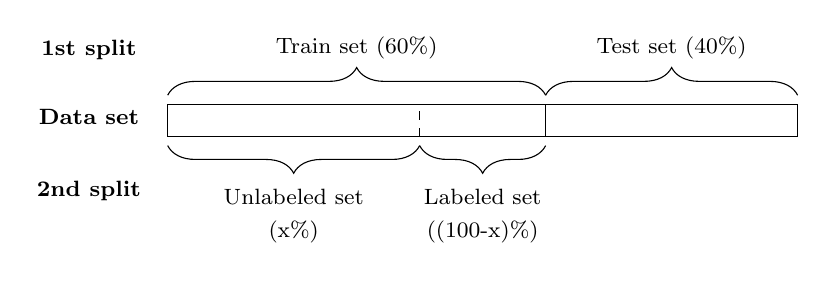
\begin{tikzpicture}[scale=0.8]
		\draw (0,0) rectangle (10,.5) node[midway]{};
		\draw (6,0) -- (6,.5);
		\draw[dashed] (4,0) -- (4,.5);
		
		\draw node[draw=none, xshift=-1cm, yshift=1.1cm] {\footnotesize \textbf{1st split}};
		\draw node[draw=none, xshift=-1cm, yshift=-.7cm] {\footnotesize \textbf{2nd split}};
		\draw node[draw=none, xshift=-1cm, yshift=.25cm] {\textbf{\footnotesize Data set}};
		
		\draw [decorate,decoration={brace,amplitude=10pt}, yshift=0.15cm]
		(0,.5) -- (6,.5) node [black,midway,yshift=0.6cm] {\footnotesize Train set (60\%)};
		\draw [decorate,decoration={brace,amplitude=10pt}, yshift=0.15cm]
		(6,.5) -- (10,.5) node [black,midway,yshift=0.6cm] {\footnotesize Test set (40\%)};
		
		\draw [decorate,decoration={brace,amplitude=10pt, mirror}, , yshift=-0.15cm]
		(0,0) -- (4,0) node [black,midway,yshift=-0.9cm, align=center] {\footnotesize Unlabeled set \\\footnotesize (x\%)};
		\draw [decorate,decoration={brace,amplitude=10pt, mirror}, yshift=-0.15cm]
		(4,0) -- (6,0) node [black,midway,yshift=-0.9cm, align=center] {\footnotesize Labeled set \\\footnotesize ((100-x)\%)};
		\end{tikzpicture}
	\end{figure}

	\pause
	
	\begin{itemize}
		\item Data: 20Newsgroup
		\item Default cross validation: 5 folds
		\item Similarity measure: Cosine for trees, Euclidean for K-means
	\end{itemize}
\end{frame}

\begin{frame}
	\frametitle{Experimental Results (Thesis Page 11)}
	Results average in f1-score with split-x, (\#labeled, \#unlabeled)
	\begin{columns}
		\column{0.5\textwidth}
		\begin{table}
			\centering
			\captionsetup{justification=centering}
			\caption{comp versus rec}
			\makebox[\textwidth][c]{
				\begin{tabular}{ ccc }
					\textbf{Random} & \textbf{Tree} & \textbf{Kmeans} \\
					\hline
					\multicolumn{3}{c}{Split-70, (1064:2484)} \\
					0.82 & 0.85 & 0.84 \pause[2]\\
					\hline
					\multicolumn{3}{c}{Split-97, (106:3442)} \\
					0.74 & 0.77 & 0.77 \\
					\hline
			\end{tabular}}
		\end{table}
		\column{0.5\textwidth}
		\pause[0]
		\begin{table}
			\centering
			\captionsetup{justification=centering}
			\caption{comp versus sci}
			\makebox[\textwidth][c]{
				\begin{tabular}{ ccc }
					\textbf{Random} & \textbf{Tree} & \textbf{Kmeans} \\
					\hline
					\multicolumn{3}{c}{Split-70, (1061:2476)} \\
					0.91 & 0.91 & 0.90 \pause[2]\\
					\hline
					\multicolumn{3}{c}{Split-97, (106:3431)} \\
					0.86 & 0.89 & 0.89 \\
					\hline
			\end{tabular}}
		\end{table}
	\end{columns}
	
	\vspace{-.5cm}
	\pause[0]
	
	\begin{table}
		\centering
		\captionsetup{justification=centering}
		\caption{comp versus talk}
		\makebox[\textwidth][c]{
			\begin{tabular}{ ccc }
				\textbf{Random} & \textbf{Tree} & \textbf{Kmeans} \\
				\hline
				\multicolumn{3}{c}{Split-70, (977:2280)} \\
				0.93 & 0.93 & 0.93 \pause[2]\\
				\hline
				\multicolumn{3}{c}{Split-97, (97:3160)} \\
				0.90 & 0.92 & 0.92\\
				\hline
		\end{tabular}}
	\end{table}
\end{frame}
